% Options for packages loaded elsewhere
\PassOptionsToPackage{unicode}{hyperref}
\PassOptionsToPackage{hyphens}{url}
\PassOptionsToPackage{dvipsnames,svgnames,x11names}{xcolor}
%
\documentclass[
  letterpaper,
  DIV=11,
  numbers=noendperiod]{scrreprt}

\usepackage{amsmath,amssymb}
\usepackage{iftex}
\ifPDFTeX
  \usepackage[T1]{fontenc}
  \usepackage[utf8]{inputenc}
  \usepackage{textcomp} % provide euro and other symbols
\else % if luatex or xetex
  \usepackage{unicode-math}
  \defaultfontfeatures{Scale=MatchLowercase}
  \defaultfontfeatures[\rmfamily]{Ligatures=TeX,Scale=1}
\fi
\usepackage{lmodern}
\ifPDFTeX\else  
    % xetex/luatex font selection
\fi
% Use upquote if available, for straight quotes in verbatim environments
\IfFileExists{upquote.sty}{\usepackage{upquote}}{}
\IfFileExists{microtype.sty}{% use microtype if available
  \usepackage[]{microtype}
  \UseMicrotypeSet[protrusion]{basicmath} % disable protrusion for tt fonts
}{}
\makeatletter
\@ifundefined{KOMAClassName}{% if non-KOMA class
  \IfFileExists{parskip.sty}{%
    \usepackage{parskip}
  }{% else
    \setlength{\parindent}{0pt}
    \setlength{\parskip}{6pt plus 2pt minus 1pt}}
}{% if KOMA class
  \KOMAoptions{parskip=half}}
\makeatother
\usepackage{xcolor}
\setlength{\emergencystretch}{3em} % prevent overfull lines
\setcounter{secnumdepth}{5}
% Make \paragraph and \subparagraph free-standing
\ifx\paragraph\undefined\else
  \let\oldparagraph\paragraph
  \renewcommand{\paragraph}[1]{\oldparagraph{#1}\mbox{}}
\fi
\ifx\subparagraph\undefined\else
  \let\oldsubparagraph\subparagraph
  \renewcommand{\subparagraph}[1]{\oldsubparagraph{#1}\mbox{}}
\fi


\providecommand{\tightlist}{%
  \setlength{\itemsep}{0pt}\setlength{\parskip}{0pt}}\usepackage{longtable,booktabs,array}
\usepackage{calc} % for calculating minipage widths
% Correct order of tables after \paragraph or \subparagraph
\usepackage{etoolbox}
\makeatletter
\patchcmd\longtable{\par}{\if@noskipsec\mbox{}\fi\par}{}{}
\makeatother
% Allow footnotes in longtable head/foot
\IfFileExists{footnotehyper.sty}{\usepackage{footnotehyper}}{\usepackage{footnote}}
\makesavenoteenv{longtable}
\usepackage{graphicx}
\makeatletter
\def\maxwidth{\ifdim\Gin@nat@width>\linewidth\linewidth\else\Gin@nat@width\fi}
\def\maxheight{\ifdim\Gin@nat@height>\textheight\textheight\else\Gin@nat@height\fi}
\makeatother
% Scale images if necessary, so that they will not overflow the page
% margins by default, and it is still possible to overwrite the defaults
% using explicit options in \includegraphics[width, height, ...]{}
\setkeys{Gin}{width=\maxwidth,height=\maxheight,keepaspectratio}
% Set default figure placement to htbp
\makeatletter
\def\fps@figure{htbp}
\makeatother
\newlength{\cslhangindent}
\setlength{\cslhangindent}{1.5em}
\newlength{\csllabelwidth}
\setlength{\csllabelwidth}{3em}
\newlength{\cslentryspacingunit} % times entry-spacing
\setlength{\cslentryspacingunit}{\parskip}
\newenvironment{CSLReferences}[2] % #1 hanging-ident, #2 entry spacing
 {% don't indent paragraphs
  \setlength{\parindent}{0pt}
  % turn on hanging indent if param 1 is 1
  \ifodd #1
  \let\oldpar\par
  \def\par{\hangindent=\cslhangindent\oldpar}
  \fi
  % set entry spacing
  \setlength{\parskip}{#2\cslentryspacingunit}
 }%
 {}
\usepackage{calc}
\newcommand{\CSLBlock}[1]{#1\hfill\break}
\newcommand{\CSLLeftMargin}[1]{\parbox[t]{\csllabelwidth}{#1}}
\newcommand{\CSLRightInline}[1]{\parbox[t]{\linewidth - \csllabelwidth}{#1}\break}
\newcommand{\CSLIndent}[1]{\hspace{\cslhangindent}#1}

\KOMAoption{captions}{tableheading}
\makeatletter
\makeatother
\makeatletter
\@ifpackageloaded{bookmark}{}{\usepackage{bookmark}}
\makeatother
\makeatletter
\@ifpackageloaded{caption}{}{\usepackage{caption}}
\AtBeginDocument{%
\ifdefined\contentsname
  \renewcommand*\contentsname{Table of contents}
\else
  \newcommand\contentsname{Table of contents}
\fi
\ifdefined\listfigurename
  \renewcommand*\listfigurename{List of Figures}
\else
  \newcommand\listfigurename{List of Figures}
\fi
\ifdefined\listtablename
  \renewcommand*\listtablename{List of Tables}
\else
  \newcommand\listtablename{List of Tables}
\fi
\ifdefined\figurename
  \renewcommand*\figurename{Figure}
\else
  \newcommand\figurename{Figure}
\fi
\ifdefined\tablename
  \renewcommand*\tablename{Table}
\else
  \newcommand\tablename{Table}
\fi
}
\@ifpackageloaded{float}{}{\usepackage{float}}
\floatstyle{ruled}
\@ifundefined{c@chapter}{\newfloat{codelisting}{h}{lop}}{\newfloat{codelisting}{h}{lop}[chapter]}
\floatname{codelisting}{Listing}
\newcommand*\listoflistings{\listof{codelisting}{List of Listings}}
\makeatother
\makeatletter
\@ifpackageloaded{caption}{}{\usepackage{caption}}
\@ifpackageloaded{subcaption}{}{\usepackage{subcaption}}
\makeatother
\makeatletter
\@ifpackageloaded{tcolorbox}{}{\usepackage[skins,breakable]{tcolorbox}}
\makeatother
\makeatletter
\@ifundefined{shadecolor}{\definecolor{shadecolor}{rgb}{.97, .97, .97}}
\makeatother
\makeatletter
\makeatother
\makeatletter
\makeatother
\ifLuaTeX
  \usepackage{selnolig}  % disable illegal ligatures
\fi
\IfFileExists{bookmark.sty}{\usepackage{bookmark}}{\usepackage{hyperref}}
\IfFileExists{xurl.sty}{\usepackage{xurl}}{} % add URL line breaks if available
\urlstyle{same} % disable monospaced font for URLs
\hypersetup{
  pdftitle={Dynamics of Youth},
  pdfauthor={Neha Moopen},
  colorlinks=true,
  linkcolor={blue},
  filecolor={Maroon},
  citecolor={Blue},
  urlcolor={Blue},
  pdfcreator={LaTeX via pandoc}}

\title{Dynamics of Youth}
\usepackage{etoolbox}
\makeatletter
\providecommand{\subtitle}[1]{% add subtitle to \maketitle
  \apptocmd{\@title}{\par {\large #1 \par}}{}{}
}
\makeatother
\subtitle{DATA HANDBOOK}
\author{Neha Moopen}
\date{2024-08-06}

\begin{document}
\maketitle
\ifdefined\Shaded\renewenvironment{Shaded}{\begin{tcolorbox}[sharp corners, frame hidden, interior hidden, breakable, enhanced, borderline west={3pt}{0pt}{shadecolor}, boxrule=0pt]}{\end{tcolorbox}}\fi

\renewcommand*\contentsname{Table of contents}
{
\hypersetup{linkcolor=}
\setcounter{tocdepth}{2}
\tableofcontents
}
\bookmarksetup{startatroot}

\hypertarget{welcome}{%
\chapter*{Welcome!}\label{welcome}}
\addcontentsline{toc}{chapter}{Welcome!}

\markboth{Welcome!}{Welcome!}

\begin{figure}

{\centering 
\includegraphics{images/fair-1x4.png}

}

\caption{This illustration is created by Scriberia with The Turing Way
community. Used under a CC-BY 4.0 licence. DOI: 10.5281/zenodo.3332807}

\end{figure}

\bookmarksetup{startatroot}

\hypertarget{data-management-plans}{%
\chapter*{Data Management Plans}\label{data-management-plans}}
\addcontentsline{toc}{chapter}{Data Management Plans}

\markboth{Data Management Plans}{Data Management Plans}

\hypertarget{what-is-a-data-management-plan}{%
\section*{What Is A Data Management
Plan?}\label{what-is-a-data-management-plan}}
\addcontentsline{toc}{section}{What Is A Data Management Plan?}

\markright{What Is A Data Management Plan?}

A Data Management Plan (DMP) is a formal document that describes your
data and outlines all aspects of managing your data - both during and
after your project.

Moreover, it is a \emph{living} document that can you can revise and
update as needed.

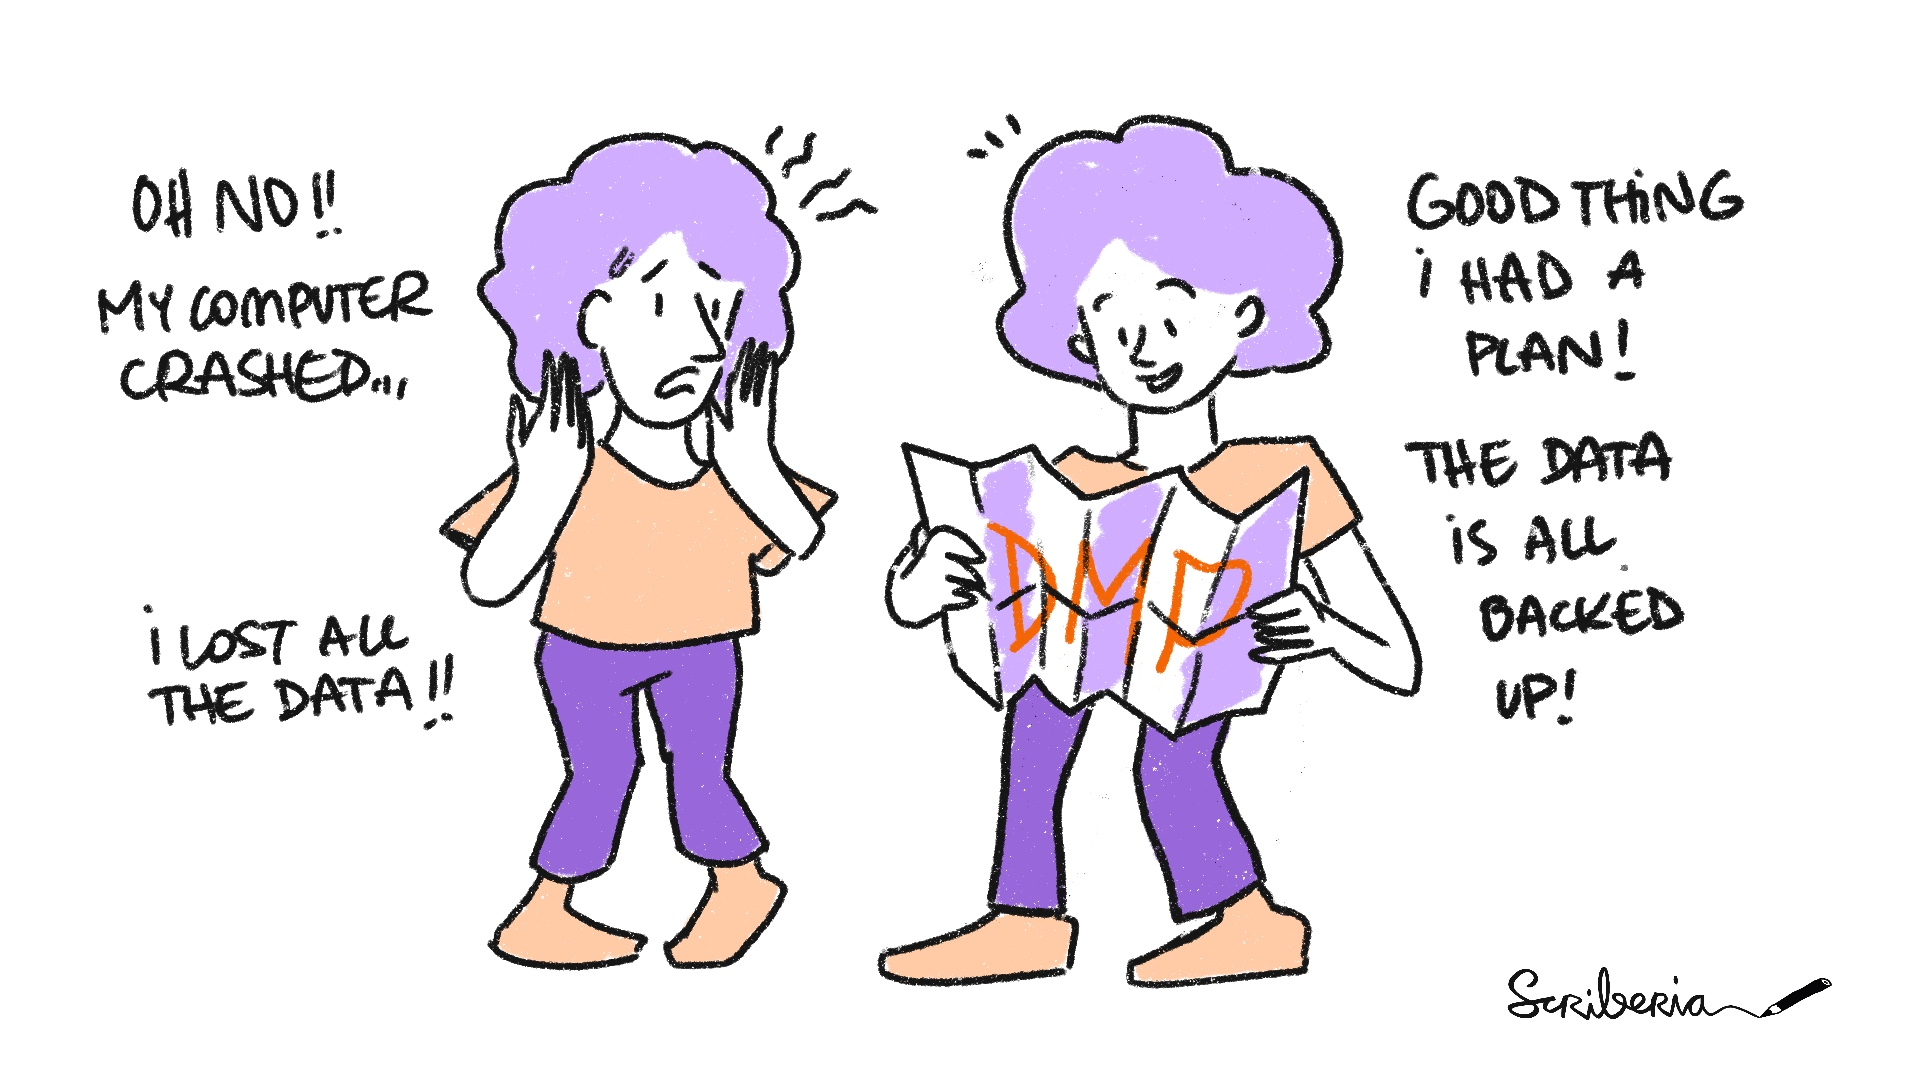
\includegraphics{images/data-management-plan.jpg}

The Turing Way project illustration by Scriberia. Used under a CC-BY 4.0
licence. DOI: 10.5281/zenodo.3332807.

\hypertarget{why-should-you-write-a-dmp}{%
\section*{Why Should You Write A
DMP?}\label{why-should-you-write-a-dmp}}
\addcontentsline{toc}{section}{Why Should You Write A DMP?}

\markright{Why Should You Write A DMP?}

Writing a DMP provides an opportunity to reflect on your data,
particularly how you organize and manage it. It nudges you to think
about how to make your RDM more \emph{concrete} and \emph{actionable}.
This creates efficiency and more value for your data.

\hypertarget{when-should-you-write-a-dmp}{%
\section*{When Should You Write A
DMP?}\label{when-should-you-write-a-dmp}}
\addcontentsline{toc}{section}{When Should You Write A DMP?}

\markright{When Should You Write A DMP?}

Working on a DMP at the start of your project will ensure that you are
better informed of best practices in RDM and prepared to implement them.
That being said, you can also write a DMP can during the project or when
it's completed.

\hypertarget{dmponline-dmp-templates}{%
\section*{DMPonline \& DMP Templates}\label{dmponline-dmp-templates}}
\addcontentsline{toc}{section}{DMPonline \& DMP Templates}

\markright{DMPonline \& DMP Templates}

DMPonline is a tool that helps you create and maintain DMPs. With
DMPonline, you can:

\begin{itemize}
\tightlist
\item
  register and sign in with your institutional credentials,
\item
  write and collaborate on (multiple) DMPs,
\item
  share DMPs or switch their visibility between private and public,
\item
  request feedback from RDM Support,
\item
  download DMPs in various formats.
\end{itemize}

DMPonline offers DMP templates from various institutions and funders,
including:

\begin{itemize}
\tightlist
\item
  Utrecht University
\item
  UMC Utrecht
\item
  \href{https://dmponline.dcc.ac.uk/template_export/1753695087.pdf}{NWO}
\item
  \href{https://dmponline.dcc.ac.uk/template_export/1461074155.pdf}{ZonMw}
\item
  \href{https://dmponline.dcc.ac.uk/template_export/2088403152.pdf}{ERC}
\item
  \href{https://dmponline.dcc.ac.uk/template_export/1612436782.pdf}{Horizon
  2020}
\item
  \href{https://dmponline.dcc.ac.uk/template_export/5992485.pdf}{Horizon
  Europe}
\end{itemize}

These templates also contain example answers and guidance.

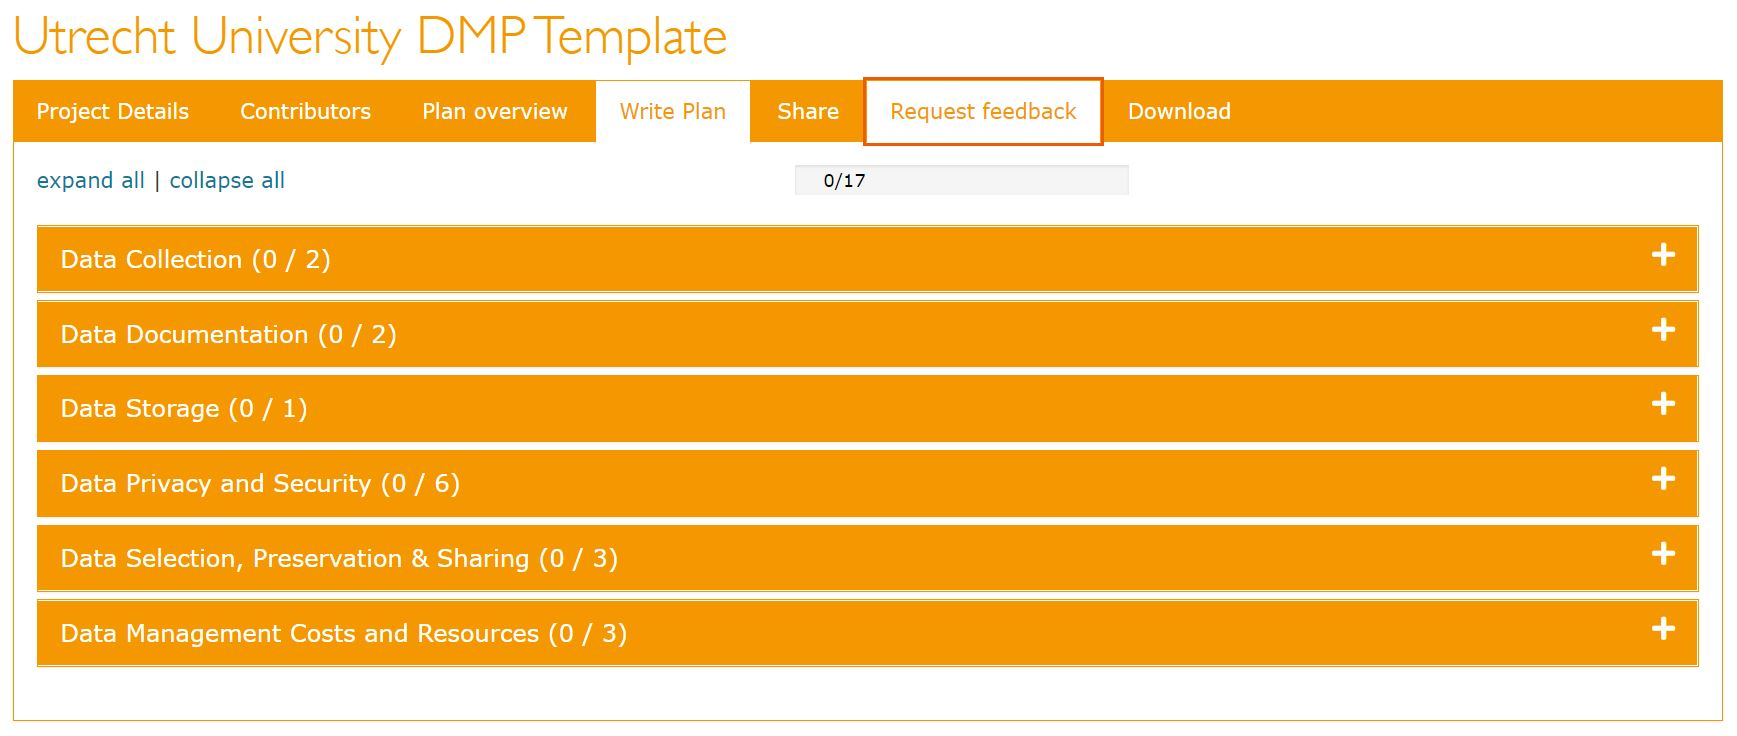
\includegraphics{images/uu-dmp-template.JPG}

\hypertarget{tips}{%
\section*{Tips}\label{tips}}
\addcontentsline{toc}{section}{Tips}

\markright{Tips}

!!! note ``Tips''

\begin{verbatim}
- Contact your DoY data manager! They can (co)write your DMP and/or review it.
- If the DoY data manager is unavailable, you can still request feedback from RDM Support.
\end{verbatim}

\hypertarget{resources}{%
\section*{Resources}\label{resources}}
\addcontentsline{toc}{section}{Resources}

\markright{Resources}

\begin{itemize}
\tightlist
\item
  \href{https://www.uu.nl/en/research/research-data-management/tools-services/tool-to-create-your-dmp-online}{Create
  your DMP online}
\item
  \href{https://www.uu.nl/en/research/research-data-management/guides/data-management-planning}{Data
  management planning}
\item
  \href{https://www.uu.nl/en/research/research-data-management/training-workshops/online-training-learn-to-write-your-dmp}{Learn
  to write your DMP (online training)}
\end{itemize}

\hypertarget{references}{%
\section*{References}\label{references}}
\addcontentsline{toc}{section}{References}

\markright{References}

\begin{enumerate}
\def\labelenumi{\arabic{enumi}.}
\item
  \url{https://www.uu.nl/en/research/research-data-management/guides/data-management-planning}
\item
  \url{https://www.kuleuven.be/rdm/en/faq/faq-dmp}
\item
  \url{https://rdm.uva.nl/en/planning/data-management-plan/data-management-plan.html}
\item
  \url{https://www.uu.nl/en/research/research-data-management/tools-services/tool-to-create-your-dmp-online.html}
\end{enumerate}

\bookmarksetup{startatroot}

\hypertarget{naming-conventions}{%
\chapter*{Naming Conventions}\label{naming-conventions}}
\addcontentsline{toc}{chapter}{Naming Conventions}

\markboth{Naming Conventions}{Naming Conventions}

\hypertarget{what-is-a-naming-convention}{%
\section*{What Is A Naming
Convention?}\label{what-is-a-naming-convention}}
\addcontentsline{toc}{section}{What Is A Naming Convention?}

\markright{What Is A Naming Convention?}

A naming convention is a set of rules for naming things. You can apply
it to things like folders, files, and variables.

\hypertarget{why-should-i-apply-a-naming-convention}{%
\section*{Why Should I Apply A Naming
Convention?}\label{why-should-i-apply-a-naming-convention}}
\addcontentsline{toc}{section}{Why Should I Apply A Naming Convention?}

\markright{Why Should I Apply A Naming Convention?}

Names that are informative and useful for machines and humans are a step
toward efficient data management and reproducible research. The more
consistent and meaningful the name, the easier it will be to locate and
identify things, understand what they contain, and (re)use them.

\hypertarget{when-should-i-apply-a-naming-convention}{%
\section*{When Should I Apply A Naming
Convention?}\label{when-should-i-apply-a-naming-convention}}
\addcontentsline{toc}{section}{When Should I Apply A Naming Convention?}

\markright{When Should I Apply A Naming Convention?}

Aim to select and implement a naming convention at the beginning of a
project. If you want to retroactively apply a naming convention, there
are several tools for bulk renaming.

The entire research team should agree on and adopt a naming convention.
Document the choice of naming convention in the DMP, so others can refer
to and grasp it quickly.

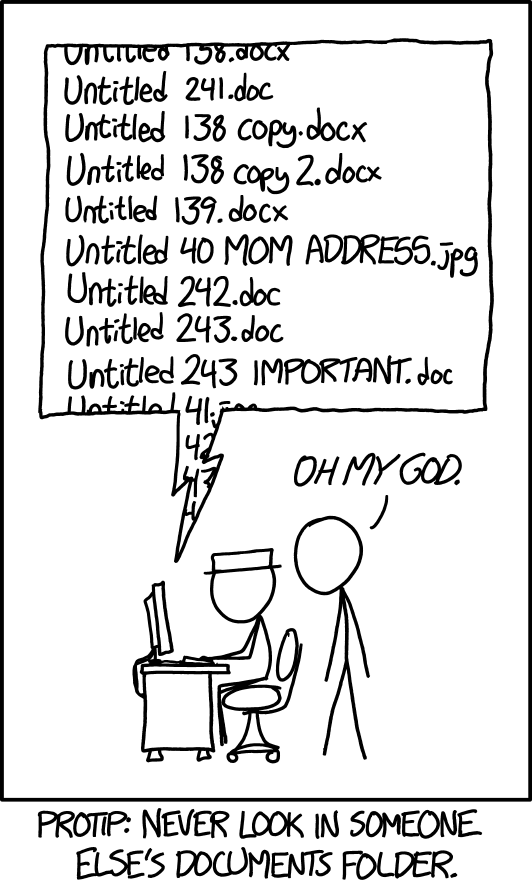
\includegraphics{images/xkcd-file-naming.png}

Documents - xkcd. Used under a CC BY-NC 2.5 license.

\hypertarget{popular-naming-conventions}{%
\section*{Popular Naming Conventions}\label{popular-naming-conventions}}
\addcontentsline{toc}{section}{Popular Naming Conventions}

\markright{Popular Naming Conventions}

Instead of developing a naming convention from scratch, you can start
with one that is already being used in programming and software
development communities:

\begin{longtable}[]{@{}
  >{\raggedright\arraybackslash}p{(\columnwidth - 4\tabcolsep) * \real{0.3636}}
  >{\raggedright\arraybackslash}p{(\columnwidth - 4\tabcolsep) * \real{0.3864}}
  >{\raggedright\arraybackslash}p{(\columnwidth - 4\tabcolsep) * \real{0.2500}}@{}}
\toprule\noalign{}
\begin{minipage}[b]{\linewidth}\raggedright
Naming Covention
\end{minipage} & \begin{minipage}[b]{\linewidth}\raggedright
Example
\end{minipage} & \begin{minipage}[b]{\linewidth}\raggedright
Description
\end{minipage} \\
\midrule\noalign{}
\endhead
\bottomrule\noalign{}
\endlastfoot
original name & \texttt{an\ awesome\ name} & N/A \\
snake\_case & \texttt{an\_awesome\_name} & All words are lowercase and
separated by an underscore ( \texttt{\_} ) \\
kebab-case & \texttt{an-awesome-name} & All words are lowercase and
separated by a hyphen ( \texttt{-} ) \\
PascalCase & \texttt{AnAwesomeName} & All words are capitalized. Spaces
are not used. \\
camelCase & \texttt{anAwesomeName} & The first word is lowercase, the
remaining words are capitalized. Spaces are not used. \\
\end{longtable}

\hypertarget{human-readable-names}{%
\section*{Human-Readable Names}\label{human-readable-names}}
\addcontentsline{toc}{section}{Human-Readable Names}

\markright{Human-Readable Names}

You can tailor naming conventions like \texttt{snake\_case} and
\texttt{PascalCase} to suit your project and workflow. Determine what
information is relevant (or not) to create meaningful names and how you
can string this information together. Don't forget to document this in
your DMP!

!!! note ``Elements for Human-Readable Names''

\begin{verbatim}
Names should be =<25 characters long and can include:

- Date of creation/update (`YYYY-MM-DD` or `YYYYMMDD`)
- Description of content, like type of data
- Initials of creator/reviewer
- Project number or acronym
- Location/coordinates
- Version number (like `v2` or v2.2`)
\end{verbatim}

\hypertarget{machine-readable-names}{%
\section*{Machine-Readable Names}\label{machine-readable-names}}
\addcontentsline{toc}{section}{Machine-Readable Names}

\markright{Machine-Readable Names}

When names are machine-readable, they can be efficiently processed by
computers and software. This makes it easier to search for files and run
operations that involve programming like extracting information from
file names or working with regular expressions.

!!! note ``Avoid''

\begin{verbatim}
- Spaces
- Special characters like `$`, `@`, `%`, `#`, `&`, `*`, `!`, `/`, `\`
- Punction characters like `,`, `:`, `;`, `?`, `'`, `"`
- Accented characters
\end{verbatim}

\hypertarget{a-note-on-numbering-dates-versioning}{%
\section*{A Note on Numbering, Dates,
Versioning}\label{a-note-on-numbering-dates-versioning}}
\addcontentsline{toc}{section}{A Note on Numbering, Dates, Versioning}

\markright{A Note on Numbering, Dates, Versioning}

\begin{itemize}
\item
  Append numbers to the beginning of a name to enable sorting according
  to a logical structure. Use multiple digits like \texttt{01} or
  \texttt{001}.
\item
  Dates should follow the ISO 8601 standard which is either
  \texttt{YYYY-MM-DD} or \texttt{YYYYMMDD}. Append dates to the
  beginning of names to enable sorting in chronological order.
\item
  Specify versions using ordinal numbers (1,2,3) for major revisions and
  decimals for minor changes (1.1, 1.2, 2.1, 2.2). Alternatively, you
  can specify versions with multiple digits like v01 and v02.
\end{itemize}

\hypertarget{renaming-files}{%
\section*{Renaming files}\label{renaming-files}}
\addcontentsline{toc}{section}{Renaming files}

\markright{Renaming files}

The following tools enable renaming in bulk:

\begin{itemize}
\tightlist
\item
  \href{https://www.bulkrenameutility.co.uk/}{Bulk Rename Utility}
  (Windows, free)
\item
  \href{https://renamer.com/}{Renamer} (MacOS, paid)
\item
  \href{https://mrrsoftware.com/namechanger/}{NameChanger}, (MacOS,
  free)
\item
  \href{https://gprename.sourceforge.net/}{GPRename} (Linux, free)
\end{itemize}

\hypertarget{references-1}{%
\section*{References}\label{references-1}}
\addcontentsline{toc}{section}{References}

\markright{References}

\begin{enumerate}
\def\labelenumi{\arabic{enumi}.}
\tightlist
\item
  \url{https://en.wikipedia.org/wiki/Naming_convention}
\item
  \url{https://help.osf.io/article/146-file-naming}
\item
  \url{https://rdm.elixir-belgium.org/file_naming.html}
\item
  \url{https://khalilstemmler.com/blogs/camel-case-snake-case-pascal-case/}
\item
  \url{https://dev.to/chaseadamsio/most-common-programming-case-types-30h9}
\item
  \url{https://rdmkit.elixir-europe.org/data_organisation}
  \url{http://dataabinitio.com/?p=987}
\item
  \url{https://dmeg.cessda.eu/Data-Management-Expert-Guide/2.-Organise-Document/File-naming-and-folder-structure}
\item
  \url{https://annakrystalli.me/rrresearchACCE20/filenaming-view.html}
\end{enumerate}

\bookmarksetup{startatroot}

\hypertarget{data-pipelining}{%
\chapter*{Data Pipelining}\label{data-pipelining}}
\addcontentsline{toc}{chapter}{Data Pipelining}

\markboth{Data Pipelining}{Data Pipelining}

A data pipeline is a series of (automated) actions that ingests raw data
from various sources and moves the data to a destination for storage and
(eventual) analysis.

Benefits of a data pipeline include:

\begin{itemize}
\tightlist
\item
  Time saved by automating the boring stuff!
\item
  Reduced mistakes.
\item
  Tasks broken down into smaller steps.
\item
  Reproducibility!
\end{itemize}

\hypertarget{when-do-i-need-a-data-pipeline}{%
\section*{When do I need a data
pipeline?}\label{when-do-i-need-a-data-pipeline}}
\addcontentsline{toc}{section}{When do I need a data pipeline?}

\markright{When do I need a data pipeline?}

Here's a rule of thumb, just as an example:

If you have a task that needs to occur \textgreater= 3 times, you could
think about automating it.

If automation is not possible, think about how you can make the task as
efficient as possible.

\hypertarget{how-can-i-implement-a-data-pipeline-some-examples-for-inspiration}{%
\section*{How can I implement a data pipeline? Some examples for
inspiration}\label{how-can-i-implement-a-data-pipeline-some-examples-for-inspiration}}
\addcontentsline{toc}{section}{How can I implement a data pipeline? Some
examples for inspiration}

\markright{How can I implement a data pipeline? Some examples for
inspiration}

\begin{itemize}
\item
  If you data collection tools have APIs, they can be leveraged to
  extract data.
\item
  For example, Qualtrics has the qualtRics R package \& pyQualtrics
  Python library which contain functions to automate exporting surveys.
\item
  If APIs are not available, you could use R/Python to automate the use
  of an internet browser using the RSelenium package / Selenium library.
  Imagine automating the clicks and typing of going to a specific
  website, logging in, clicking the download button.
\item
  You can use Windows Task Scheduler / cron / the taskscheduleR R
  package / cronR to schedule your scripts to run automatically, on a
  recurring basis as well (if needed).
\item
  You can also send emails with R \& Python! Consider if you've ever had
  to contact participants because you noticed something wrong with their
  incoming data. You could implement these data checks with a script and
  automatically draft and send emails (from a template) to those
  participants who were flagged as having issues with their data.
\end{itemize}

\hypertarget{qualtrics-r-package}{%
\section*{QualtRics R package}\label{qualtrics-r-package}}
\addcontentsline{toc}{section}{QualtRics R package}

\markright{QualtRics R package}

\begin{verbatim}
library(readr)
library(qualtRics)

qualtrics_api_credentials(api_key = "YOUR-QUALTRICS-API-KEY", 
                          base_url = "YOUR-QUALTRICS-BASE-URL",
                          overwrite = TRUE,
                          install = TRUE)

readRenviron("~/.Renviron")

surveys <- all_surveys() 

survey_results <- fetch_survey(surveyID = surveys$id[2], # you can also replace surveys$id[2] with "<SUVREY-ID>" 
                                  verbose = TRUE)

write_csv(survey_results, paste0("path/to/folder/", format(Sys.time(), "%d-%m-%Y-%H.%M"), "_survey_results.csv"))
\end{verbatim}

\hypertarget{taskscheduler-package}{%
\section*{taskscheduleR package}\label{taskscheduler-package}}
\addcontentsline{toc}{section}{taskscheduleR package}

\markright{taskscheduleR package}

\begin{verbatim}
library(taskscheduleR)

scheduled_script <- "path/to/folder/myscript.R"

## run script once within 120 seconds

taskscheduler_create(taskname = "extract-data-once", rscript = scheduled_script,
                     schedule = "ONCE", starttime = format(Sys.time() + 120, "%H:%M"))

## Run every 5 minutes, starting from 10:40

taskscheduler_create(taskname = "extract-data-5min", rscript = scheduled_script,
                     schedule = "MINUTE", starttime = "10:40", modifier = 5)

## delete tasks

taskscheduler_delete("extract-data-once")
\end{verbatim}

\bookmarksetup{startatroot}

\hypertarget{codebooks}{%
\chapter*{Codebooks}\label{codebooks}}
\addcontentsline{toc}{chapter}{Codebooks}

\markboth{Codebooks}{Codebooks}

A codebook is an example of data-level metadata.

The purpose of a codebook or data dictionary is to explain what all the
variable names and values in your spreadsheet really mean.

Information to include in a codebook includes:

\begin{itemize}
\tightlist
\item
  Variable Names
\item
  Readable Variable Name
\item
  Measurement Units
\item
  Allowed Values
\item
  Definition Of The Variable
\item
  Synonyms For The Variable Name (Optional)
\item
  Description Of The Variable (Optional)
\item
  Other Resources
\end{itemize}

See: \url{https://help.osf.io/article/217-how-to-make-a-data-dictionary}

\hypertarget{codebook-r-package}{%
\section*{codebook R package}\label{codebook-r-package}}
\addcontentsline{toc}{section}{codebook R package}

\markright{codebook R package}

\begin{verbatim}
library(qualtRics)
library(readr)
library(dplyr)
library(codebook)
library(writexl)

surveys <- all_surveys()

survey_results <- fetch_survey(surveyID = surveys$id[2], # you can also replace surveys$id[2] with "<SUVREY-ID>"
                               verbose = TRUE)

survey_results <- select(survey_results, -c(1:17))

# survey_questions() retrieves a data frame containing questions and question IDs for a survey;
survey_questions <- survey_questions(surveyID = surveys$id[2])
survey_questions <- select(survey_questions, -c(1, 4))
survey_questions <- slice(survey_questions, -1)
  
# generate codebook

codebook <- codebook_table(survey_results)

codebook <- rename(codebook, qname = name)

codebook <- full_join(survey_questions, codebook, by = "qname")

write_xlsx(codebook, "documentation/codebook-demo.xlsx")
\end{verbatim}

The \texttt{labelled} R package can also do something similar.

\bookmarksetup{startatroot}

\hypertarget{references-2}{%
\chapter*{References}\label{references-2}}
\addcontentsline{toc}{chapter}{References}

\markboth{References}{References}

\hypertarget{refs}{}
\begin{CSLReferences}{0}{0}
\end{CSLReferences}



\end{document}
